\documentclass[finalProposal.tex]{subfiles}
\begin{document}
\onehalfspacing

\noindent{\Large Technical Documentation}

\bigskip

The GSR circuit's schematic is included below where the output of the last op-amp goes to Analog Pin 1 on the Arduino instead of through an LED as shown. V+ is connected to the 5V output pin of 
the Arduino and V- (or V as it is mislabeled in one place) goes to the ground pin of the Arduino. The nodes labeled skin-1 and skin-2 go to the finger probes that just consist of a conductive metal 
strip of aluminum glued to a velcro strap that allows the probe to be tightened around the finger.

\begin{center}
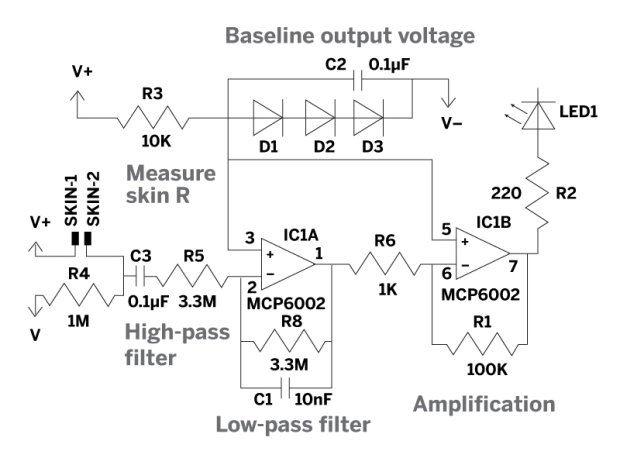
\includegraphics[scale=0.5]{gsrCircuit.jpg} \\
\emph{Circuit diagram of GSR circuit} [1]
\end{center}

The heartbeat monitor circuit is an integrated circuit that was purchased from Sparkfun Electronics. The outputs are labeled as +V which connects to the 5V pin of the Arduino, GND which connects to
the ground pin, and OUT which connects to Analog Pin 0 of the Arduino. This integrated circuit was also attached to a velcro strap so that it could be mounted on a finger and is easily adjustable. 
The schematic from Sparkfun is shown below:

\begin{center}
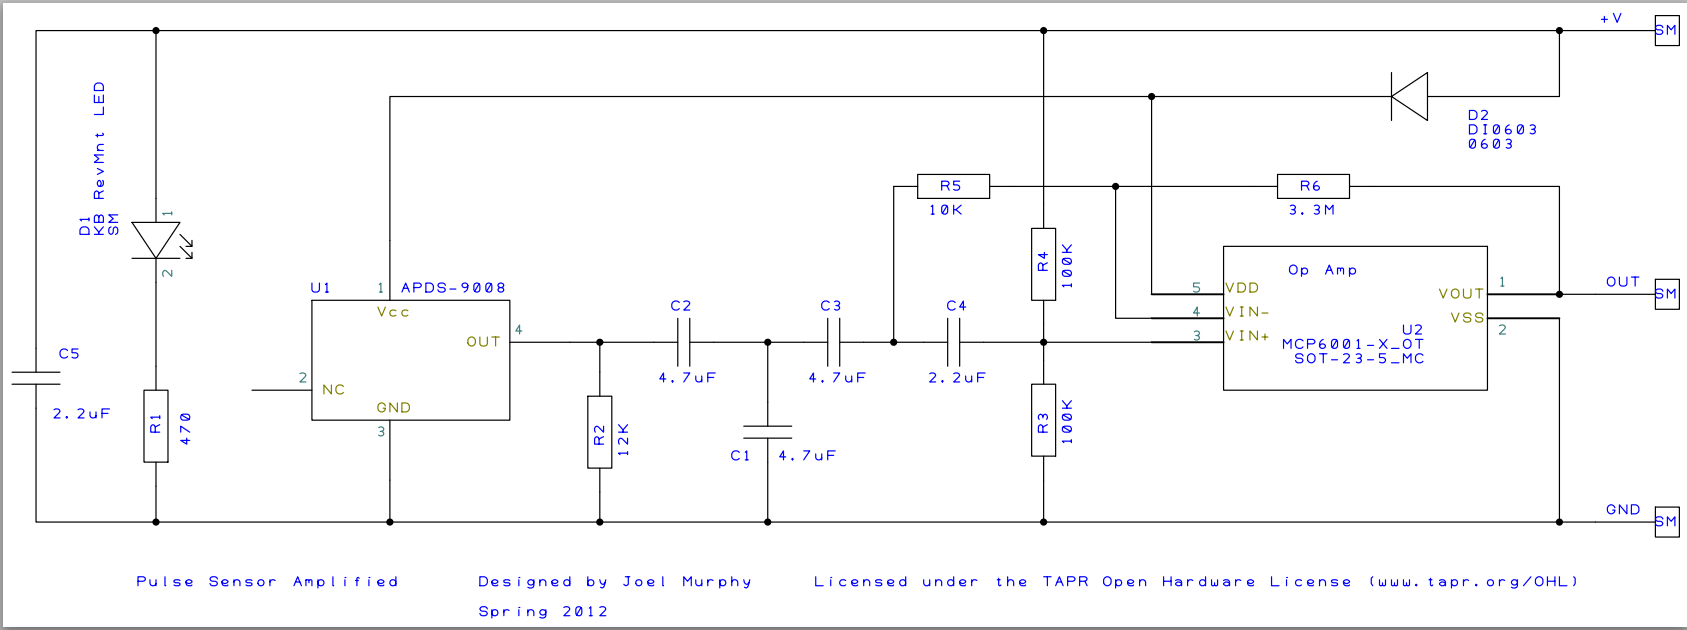
\includegraphics[scale=0.4]{pulseSensorSchematic.PNG} \\
\emph{Circuit schematic of heart beat sensor} [2]
\end{center}

The bluetooth module is then connected to the Arduino. The power and ground go the 5V and ground pins of the Arduino respectfully. The Rx goes to pin 3 and the Tx goes to pin 2 which are defined in
the software to be the Tx and Rx pins of the Arduino.

These are all of the external circuits. The flow of data is from the probes to the GSR and heartbeat circuits which is an analog value. This analog value is converted to a digital signal and processed
on the Arduino. Then the processed, digital value is sent to the bluetooth module and transmitted to the android application where it is collected and graphed.

\end{document}
